%
% teil1.tex -- Beispiel-File für das Paper
%
% (c) 2020 Prof Dr Andreas Müller, Hochschule Rapperswil
%
%
% teil2.tex -- Beispiel-File für teil2 
%
% (c) 2020 Prof Dr Andreas Müller, Hochschule Rapperswil
%


\section{Kalman Filter}
\subsection{Geschichte}
Das Kalman Filter wurde 1960 von Rudolf Emil Kalman entdeckt und direkt von der NASA für die Appollo Mission benutzt. Der Filter kommt mit wenig Rechenleistung aus und war somit dafür geeignet die Rakete bei der Navigation zu unterstützen. Das Filter schätzt den Zustand eines Systems anhand von Messungen und kann den nächsten Zustand errechnen. Typische Anwendungen des Kalman-Filters sind die Glättung von verrauschten Daten und die Schätzung von Parametern und kommt heutzutage in jedem Satellit, Navigationssystem, Smartphones und Videospielen vor.

\subsection{Wahrscheinlichkeit}
Das Kalman-Filter schätzt den wahrscheinlichsten Wert zwischen zwei Normalverteilungen oder auch Gauss-Verteilung. Die eine Kurve zeigt die errechnete Vorhersage des Zustands, bzw. deren Normalverteilung. Die andere Kurve zeigt die verrauschte Messung des nächsten Zustand, bzw. deren Normalverteilung. Wie man am Beispiel dieser zwei Gauss-Verteilungen sehen kann, ist sowohl der geschätzte Zustand als auch der gemessene Zustand verteilt und haben unterschiedliche Standardabweichungen $\sigma$ und Erwartungswerte $\mu$.



\begin{figure}
 \begin{center}
 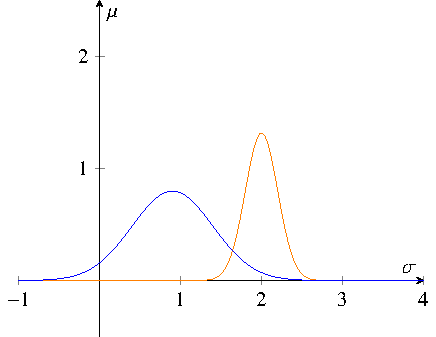
\includegraphics[width=5cm]{papers/erdbeben/Gausskurve2.pdf}
 \caption{System}
 \end{center}
\end{figure}



Um eine genauere Schätzung des Zustandes zu machen, wird nun ein Wert zwischen den beiden Verteilungen gesucht. An diesem Punkt wird nun eine Eigenschaft ausgenutzt. Durch das Multiplizieren zweier Normalverteilungen entsteht eine neue Normalverteilung. 

Wir haben eine Normalverteilung der Vorhersage:
\begin{equation}
{y_1}(x;{\mu_1},{\sigma_1})=\frac{1}{\sqrt{2\pi\sigma_1^2}}\quad e^{-\frac{(x-{\mu_1})^2}{2{\sigma_1}^2}}
\end{equation} 
und für die Messung:

\begin{equation}
{y_2}(x;{\mu_2},{\sigma_2})=\frac{1}{\sqrt{2\pi\sigma_2^2}}\quad e^{-\frac{(x-{\mu_2})^2}{2{\sigma_2}^2}}.
\end{equation} 

Diesen werden nun Multipliziert und durch deren Fläche geteilt um sie wieder zu Normieren:
\begin{equation}
{y_f}(x;{\mu_f},{\sigma_f})=\frac{ \frac{1}{\sqrt{2\pi\sigma_1^2}}e^{-\frac{(x-{\mu_1})^2}{2{\sigma_1}^2}} \cdot \frac{1}{\sqrt{2\pi\sigma_2^2}}e^{-\frac{(x-{\mu_2})^2}{2{\sigma_2}^2}}}{\int {y_1}*{y_2} dx\,}
\end{equation} 

Dadurch gleicht sich die neue Kurve den anderen an. Interessant daran ist, dass die fusionierte Kurve sich der genauere Normal-Verteilung anpasst. ist ${\sigma_2}$ klein und ${\sigma_1}$ gross, so wird sich die fusionierte Kurve näher an ${y_2}(x;{\mu_2},{\sigma_2})$ begeben. Sie ist also gewichtet und die best mögliche Schätzung. 


\begin{figure}
 \begin{center}
 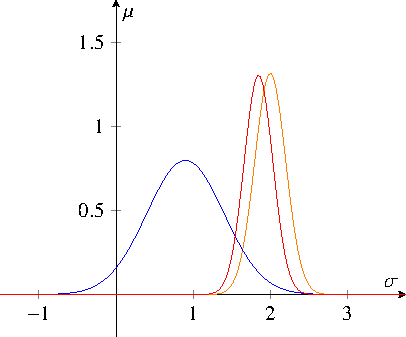
\includegraphics[width=5cm]{papers/erdbeben/Gausskurve3.pdf}
 \caption{System}
 \end{center}
\end{figure}

 
Was in 2 Dimensionen erklärt wurde, funktioniert auch in mehreren Dimensionen. Dieses Prinzip mach sich der Kalman Filter zu nutze, und wird von uns für die Erdbeben Berechnung genutzt. 




\section{Aufbau}
Um ein Erdbeben kenntlich zu machen werden in der Regel Seismographen mit vielen Sensoren verwendet. 
Ein Seismograph besteht im Grunde aus einer federgelagerten Masse. Wirkt eine Bodenerregung auf das Gerät ein, bleibt die gekoppelte Masse stehen und das Gehäuse schwingt mit.Relativbewegung des Bodens kann damit als Längenänderung im Zeitverlauf gemessen werden. In modernen Seismographen wird die Bodenbewegung in alle Richtungen gemessen, sowohl Horizontal als auch Vertikal. 
Wir konstruieren uns eine einfachere Version eines Seismographen, welcher rein mechanisch funktioniert. Zudem kann er nur in eine Dimension Messwerte aufnehmen. Würde das System ausgebaut werden, um alle Horizontalbewegungen aufzunehmen, würde der Verwendung des Kalman-Filters zu kompliziert werden. Für zwei Dimensionen (x,y) würde der Pythagoras für das System benötigt werden. Da sich der Pythagoras bekanntlich nicht linear verhält, kann kein lineares Kalman-Filter implementiert werden. Da das Kalman-Filter besonders effektiv und einfach für lineare Abläufe geeignet ist, würde eine Zweidimensionale Betrachtung den Rahmen dieser Arbeit sprengen. Für ein nicht-lineares System werden Extended Kalman-Filter benötigt, bei denen die System-Matrix (A) durch die Jacobi-Matrix des System ersetzt wird. Einfachheitshalber beschränken wir uns aber auf den linearen Fall, da dadurch die wesentlichen punkte bereits aufgezeigt werden. 

\begin{figure}
 \begin{center}
 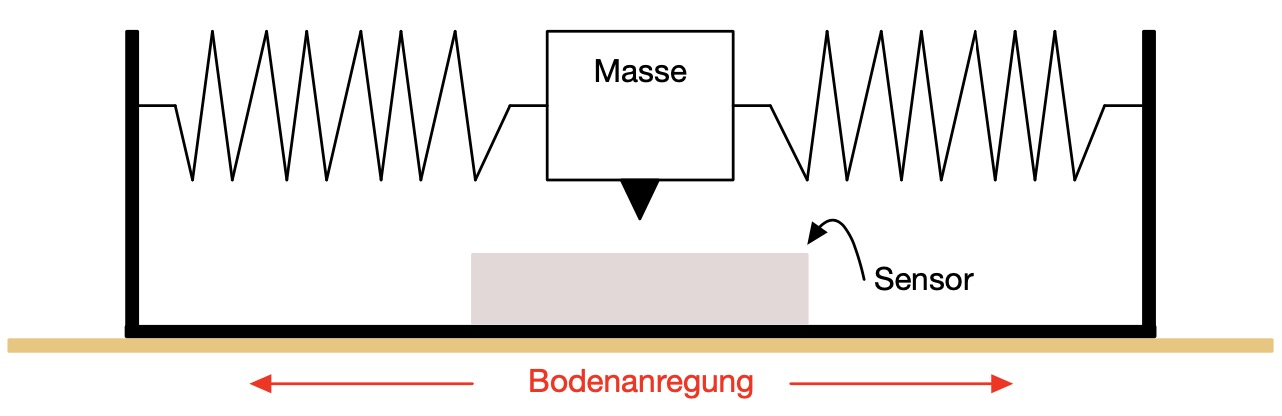
\includegraphics[width=5cm]{papers/erdbeben/Apperatur}
 \caption{System}
 \end{center}
\end{figure}



\section{Systemgleichung}
Da das Kalman-Filter zum Schätzen des nächsten Zustand verwendet wird, benötigt das Kalman-Filter eine Beschreibung der Systemdynamik. Im Fall unseres Seismographen, kann die Differentialgleichung zweiter Ordnung einer gedämpften Schwingung am harmonischen Oszillator verwendet werden. Diese lautet:
\begin{equation}
m\ddot x + 2k \dot x + Dx = f
\end{equation}
mit den Konstanten $m$ = Masse, $k$ = Dämpfungskonstante und $D$  = Federkonstante.

Um diese nun in die Systemmatrix umzuwandeln, wird aus der Differentialgleichung zweiter Ordnung durch die Substitution 
\[ {x_1}=x, \qquad
{x_2}=\dot x,  \qquad
{x_3}=\ddot x\qquad\]
erhalten wir die Differentialgleichung
\[ m{x_3}+ 2k{x_2} + D{x_1} = f.\]
Diese können wir nun in der Form
\[ {x_3}=-\frac{D}{m} {x_1} -\frac{2k}{m} {x_2} + \frac{f} {m} \]
auch als Matrix-Vektor-Gleichung darstellen.


Dafür wird die Gleichung in die Zustände aufgeteilt. Die für uns relevanten Zustände sind die Position der Masse, die Geschwindigkeit der Masse und die äussere Beschleunigung des ganzen System. Dabei muss unterschieden werden, um welche Beschleunigung es sich handelt. Das System beinhaltet sowohl eine Beschleunigung der Masse bzw. Feder (innere Beschleunigung), als auch eine Beschleunigung der ganzen Apparatur (äussere Beschleunigung). In unserem Fall wird die äusseren Beschleunigung gesucht, da diese der Erdbeben Anregung gleich kommt. 


\begin{equation}
\frac{d}{dt} \left(\begin{array}{c} {x_1} \\ {x_2}  \end{array}\right) = \left(
 \begin{array}{ccc} 	
0 & 1& 0 \\ 
- \frac{D}{m} &-\frac{2k}{m} & \frac{1} {m}\\
\end{array}\right)  \left(\begin{array}{c} {x_1} \\ {x_2} \\ {x_3} \end{array}\right).
\end{equation}

Durch die Rücksubstituion ergibt sich:
\begin{equation}
\frac{d}{dt} \left(\begin{array}{c} x(t) \\ v(t) \end{array}\right) = \left(
 \begin{array}{ccc} 	
0 & 1& 0 \\ 
- \frac{D}{m} &-\frac{2k}{m} & \frac{1} {m}\\
\end{array}\right)  \left(\begin{array}{c} x(t)\\ v(t)\\ f(t) \end{array}\right).
\end{equation}


Da die Kraft unbekannt ist, wird die letzte Zeile später mit Nullen bestückt, denn genau diese Werte wollen wir. 

\section{Kalman Filter}
Um den Kalman Filter zu starten, müssen gewisse Bedingungen definiert werden. In diesem Abschnitt werden die einzelnen Parameter/Matrizen erläutert und Erklärt, wofür sie nützlich sind. 


\subsection{Anfangsbedingungen}
\subsubsection*{Anfangszustand $x$}
Das Filter benötigt eine Anfangsbedingung. In unserem Fall ist es die Ruhelage, die Masse bewegt sich nicht. Zudem erfährt die Apparatur keine äussere Kraft.

\begin{equation}
{x_0 }= \left( \begin{array}{c} 0\\ 0\\ 0\end{array}\right)
\end{equation} 

\subsubsection*{Anfangsfehler / Kovarianzmatrix $P$}
Da auch der Anfangszustand fehlerhaft sein kann, wird für den Filter einen Anfangsfehler eingeführt. Auf der Diagonalen werden die Varianzen eingesetzt, in den restlichen Felder stehen die Kovarianzen.
Zur Erinnerung: Die Varianz ist ein Mass für die Streuung eines Wertes, die Kovarianz hingegen beschreibt die Abhängigkeit der Streuungen zweier Werte.

Kovarianz: Cov(x, y) undVarianz: Var(x) = Cov(x, x)

In unserem Fall ist der Anfangszustand gut bekannt. Wir gehen davon aus, dass das System in Ruhe und in Abwesenheit eines Erdbeben startet, somit kann die Matrix mit Nullen bestückt werden. Somit ergibt sich für die Kovarianzmatrix

\begin{equation}
{P_0 }=
\left(
\begin{array}{ccc} 	
0 & 0 &0 \\ 
0 &0 & 0 \\ 
0 & 0 &0 \\
\end{array}
\right).
\end{equation}
Diese Matrix beschreibt die Unsicherheit des geschätzten Zustandes und wird sowohl für die Vorhersage als auch die Korrektur benötigt. Sie wird nach jeder Schätzung aktualisiert.. Für einen gut bekannten Zustandsvektor können kleine Werte eingesetzt werden, für ungenaue Anfangsbedingungen sollten grosse Werte (1 Million) verwendet werden. Grosse Werte ermöglichen dem Filter sich schnell einzupendeln. 


\subsubsection*{Dynamikmatrix $A$}
Die Dynamikmatrix bildet den Kern des Filters. Diese wurde weiter oben Bereits beschrieben. Dabei wollen wird die äussere Kraft des Systems ermitteln.
Da nichts über die äussere Kraft bekannt ist, müssen wir annehmen das deren Ableitung 0 ist.
Die System Vektor-Gleichung lautet daher:


\begin{equation}
A = \left(
 \begin{array}{ccc} 	
0 & 1& 0 \\
- \frac{D}{m} &-\frac{2k}{m} & \frac{1} {m}\\
0 & 0& 0\\ 
\end{array}\right)  
\end{equation} 

\subsubsection*{Prozessrauschkovarianzmatrix $Q$}
Die Prozessrauschmatrix teilt dem Filter mit, wie sich der Systemzustand verändert. Kalman-Filter berücksichtigen Unsicherheiten wie Messfehler und -rauschen. Bei unserem Modell könnte das beispielsweise ein Windstoss an die Masse sein. Für uns wäre dies:
\begin{equation}
Q = \left(
 \begin{array}{ccc} 	
{\sigma_x }^2& 0& 0 \\ 
0 & {\sigma_v }^2& 0\\ 
0 & 0& {\sigma_f }^2\\
\end{array}\right)  
\end{equation} 

Die Standabweichungen müssten Statistisch ermittelt werden, da der Fehler nicht vom Sensor kommt und somit nicht vom Hersteller gegeben ist. Das Bedeutet wiederum dass $Q$ die Unsicherheit des Prozesses beschreibt, und die der Messung. 

\subsubsection*{Messmatrix $H$}
Die Messmatrix gibt an, welche Parameter gemessen werden soll. In unserem Falle ist es nur die Position der Massen. 

\[ H = (1, 0, 0) \]


\subsubsection*{Messrauschkovarianz $R$}
Die Messrauschkovarianzmatrix beinhaltet, wie der Name es schon sagt, das Rauschen der Positionssensoren. In unserem Fall wird nur die Position der Masse gemessen. Da wir keine anderen Sensoren haben ist $R$ lediglich:
\begin{equation}
R= ({\sigma_x}^2).
\end{equation} 
Diese Messrauchen wird meistens vom Sensorhersteller angegeben. Für unsere Theoretische Apparatur wird hier ein kleiner Fehler eingesetzt.

\subsection{Fiter Algorithmus}
Nachdem alle Parameter aufgestellt sind, wird der Filter initialisiert und wird den Zustand der Feder vorherzusagen, die Messung zu präzisieren und laufend zu aktualisieren. Das Filter berechnet aufgrund der aktuellen Schätzung eine Vorhersage. Diese wird, sobald verfügbar, mit der Messung verglichen. Aus dieser Differenz und den Unsicherheiten des Prozesses ($Q$) und der Messung ($R$) wird der wahrscheinlichste, neue Zustand geschätzt.


\subsubsection*{Vorhersage}
Im Filterschritt Vorhersage wird der nächste Zustand anhand des Anfangszustand und der Systemmatrix berechnet. Dies funktioniert mit dem Rechenschritt:
\begin{equation}
{x_{t+1}}=A\cdot{x_t}.
\end{equation} 


Die Kovarianz $P_{pred}$ wird ebenfalls neu berechnet. Da wir ein mehrdimensionales System haben, kommt noch die Prozessunsicherheit $Q$ dazu, so dass die Unsicherheit des Anfangsfehlers $P$ laufend verändert. Dies funktioniert durch multiplizieren der Systemmatrix mit dem aktualisierten Anfangsfehler. Dazu wird noch die Prozessunsicherheit addiert, somit entsteht die Gleichung
\[ P_\mathrm{pred} = A P A^T + Q . \]

wird dieser Vorgang wiederholt, schaut der Filter wie genau die letzte Anpassung von $P$ zur Messung stimmt. Ist der Unterschied klein, wird die Kovarianz $P$ kleiner, ist der Unterschied gross, wird auch die Kovarianz grösser. Das Filter passt sich selber an und korrigiert sich bei grosser Abweichung.

\subsubsection*{Messen}
Der Sensor wurde noch nicht benutz, doch genau der liefert Werte für den Filter. Die aktuellen Messwerte $z$ werden die Innovation $w$ mit dem Zustandsvektor $x$ und der Messmatrix $H$ zusammengerechnet.
Hier bei wird lediglich die Messung mit dem Fehler behaftet, und die Messmatrix $H$ 
\begin{equation}
w=Z-(H\cdot x)
\end{equation}
Die Innovation ist der Teil der Messung, die nicht durch die Systemdynamik erklärt werden kann. Die Hilfsgröße Innovation beschreibt, wie genau der vorhergesagte Mittelwert den aktuellen Messwert mittels der Beobachtungsgleichung beschreiben kann. Für eine schlechte Vorhersage wird die dazugehörige Innovation gross, für eine genaue Vorhersage dagegen klein sein. Entsprechende Korrekturen müssen dann gross bzw. nur gering ausfallen. Innovation = Messung - Vorhersage. Dies ist intuitiv logisch, eine Innovation von 0 bedeutet, dass die Messung nichts Neues hervorbrachte.

Im nächsten Schritt wir analysiert, mit welcher Kovarianz weiter gerechnet wird. 
Hierbei wird die Unsicherheit $P$, die Messmatrix $H$ und die Messunsicherheit $R$ miteinander verrechnet. 
\begin{equation}
S=Z-(H\cdot P\cdot H`+R)
\end{equation}


\subsubsection*{Aktualisieren}
Im nächsten Schritt kommt nun die Wahrscheinlichkeit nach Gauss dazu. 

\begin{equation}
K= \frac{P \cdot H`}S
\end{equation}
Dieser Vorgang wird Kalman-Gain genannt. Er sagt aus, welcher Kurve mehr Vertraut werden soll, dem Messwert oder der Systemdynamik.
Das Kalman-Gain wird geringer wen der Messwert dem vorhergesagten Systemzustand entspricht. Sind die Messwerte komplett anders als die Vorhersage, wo werden die Elemente in der Matrix $K$ grösser.

Anhand der Informationen aus dem Kalman-Gain $K$ wird das System geupdated.

\begin{equation}
x=x+(K \cdot w) 
\end{equation}

Dazu kommt  eine neue Kovarianz für den nächste Vorhersageschritt:

\begin{equation}
P=(I-(K \cdot H)) \cdot P  
\end{equation}

Der ganze Ablauf wird nun zum Algorithmus und beginnt wieder mit der Vorhersage 

\begin{equation}
{x_{t+1}}=e^{A\Delta t}{ x_t}.
\end{equation} 


\subsection{Zusammenfassung }
Zusammenfassend kann das Kalman-Filter in offizieller Typus dargestellt werden. Dabei beginnt das Filter mit dem Anfangszustand für $k=0$

1. Nächster Zustand vorhersagen
\begin{equation}
{x_{k|k-1}}={A_{k-1}}{x_{k-1}}+{B_{k-1}}{u_{k-1}}
\end{equation} 

2. Nächste Fehlerkovarianz vorhersagen
\begin{equation}
{P_{k|k-1}}={A_{k-1}}{P_{k-1}}{A_{k-1}^T}+{Q_{k-1}}
\end{equation} 


3. Das Kalman Filter anwenden
\begin{equation}
{K_k}={P_{k-1}}{H_{k}^T({H_k}{P_{k|k-1}}{H_k}^T}+{R_k})^{-1}
\end{equation}

4. Schätzung aktualisieren
\begin{equation}
{x_k}={x_{k|k-1}}+{K_k}({z_k}-{H_k}{x_{k|k-1}})
\end{equation}  

5. Fehlerkovarianz aktualisieren
\begin{equation}
{P_k}=(I-{K_k}{H_k}){P_{k|k-1}}
\end{equation}  

6. Die Outputs von $k$ werden die Inputs für ${k-1}$ und werden wieder im Schritt 1 verwendet


\section{Matlab-Code}
Um das simulierte Erdbeben auf die theoretische Apparatur zu bringen und mit dem Kalman-Filter Resultate zu generieren, wurde in Matlab der Algorithmus programmiert. 
\begin{lstlisting}
%% Initialisierte Werte
t0      =  0.00; % Anfangszeit
deltat  =  0.01; % Zeitschritt
tend    = 50.00; % Endzeit

% Standard-Abweichungen Prozess
sigmax = 0.05e-3;  % Position
sigmav = 0.01e-3;  % Geschwindigkeit
sigmaf = 1;        % (Äussere) Kraft

% Standard-Abweichung Messung
sigmam = 0.01e-3;

% Systemparameter
m = 1.00; % Masse
D = 0.30; % Federkonstante
k = 0.10; % Dämpfung


%% Kalmanfilter
% Initialisierung


% Anfangszustand (Position, Geschwindigkeit, Kraft)
x0 = [0; 0; 0];

% Unsicherheit des Anfangszustand
P0 = [0, 0, 0; ...
      0, 0, 0; ...
      0, 0, 0];

% Systemmatrizen
A = [0, 1, 0;...             %   Dynamikmatrix
    -D/m, -2*k/m, 1;...      
    0, 0, 0];                %   Ableitungen von f(t) unbekant. Annahme: 0
A = expm(A * deltat);

Q = [sigmax^2, 0, 0;...      
    0, sigmav^2, 0;...
    0, 0, sigmaf^2];         %   Prozessrauschen (Covarianz)

% Messprozess
H = [1, 0, 0];  % Messmatrix
R = sigmam^2;   % Messrauschen  (Könnte durch Versuche bestimmt werden)

I = eye(3);          % Identity matrix  (Einheitsmatrix)

% Filterprozess

% Initialisieren der Variablen
N     = length(t);    % Anzahl Punkte im Einheitsvektor (= Anzahl Messwerte)
xhat  = zeros(3, N);  % Matrix mit geschätzten Zuständen

% Index ':' bedeutet:      'alles'
% Index '(1, :)' bedeutet: 'alles aus der 1. Zeile'

% Anfangszustand setzen
xhat(:, 1) = x0; 
P = P0;

% Kalman-Matrizen konvergiert. Vorab-Berechnung in 'genügenden' Iterationen
for idx = 1:100
  Ppred = A * P * A' + Q;   % Prädizieren der Kovarianz
  S = (H * Ppred * H' + R); % Innovationskovarianz
  K = Ppred * H' / S;       % Filter-Matrix (Kalman-Gain)
  P = (I - K * H) * Ppred;  % Aktualisieren der Kovarianz  
end

% Anfangszustand gegeben
% Erster zu berechnender Wert ist der zweite
for idx = 2:N
  % Vorhersage
  xpred = A * xhat(:, idx-1);   % Prädizierter Zustand aus Bisherigem und System
  % Ppred = A * P * A' + Q;   % Prädizieren der Kovarianz

  % Korrektur
  y = xt(idx) - H * xpred;        % Messungen/ Kraft aus System - Vohersage
  % S = (H * Ppred * H' + R);     % Innovationskovarianz
  % K = Ppred * H' / S;           

  xhat(:, idx) = xpred + K * y;    % Aktualisieren des Systemzustands
  % P = (I - K * H) * Ppred;       % Aktualisieren der Kovarianz
end
\end{lstlisting}






